\documentclass[letterpaper, 8pt]{extarticle}
\usepackage{amssymb,amsmath,amsthm,amsfonts}
\usepackage{multicol,multirow}
\usepackage{calc}
\usepackage{ifthen}
\usepackage[landscape]{geometry}
\usepackage[colorlinks=true,citecolor=blue,linkcolor=blue]{hyperref}

\usepackage{booktabs}
\usepackage{ulem}
\usepackage{enumitem}
\usepackage{tabulary}
\usepackage{graphicx}
\usepackage{siunitx}
\usepackage{tikz}
\usepackage{derivative}
\usepackage{svg}
\usepackage{listings}
\usepackage{setspace}
\usepackage{listings}
\usepackage{xcolor}
\usepackage{courier}
\usepackage{syntax}
\usepackage{mathpartir}
\usepackage{braket}

% minimal line spacing
% \setstretch{0.1}

% set borders (experimentally determined to minimize cutoff and maximize space on school printers)
\geometry{top=.25in,left=.25in,right=.25in,bottom=.35in}

% make figures work better in multicol
% \newenvironment{Figure}
% {\par\medskip\noindent\minipage}
% {\endminipage\par\medskip}

% \pagestyle{empty} % clear page

% rewrite section commands to be smaller
\makeatletter
\renewcommand{\section}{\@startsection{section}{1}{0mm}%
                                {-1explus -.5ex minus -.2ex}%
                                {0.5ex plus .2ex}%x
                                {\normalfont\normalsize\bfseries}}
\renewcommand{\subsection}{\@startsection{subsection}{2}{0mm}%
                                {-1explus -.5ex minus -.2ex}%
                                {0.5ex plus .2ex}%
                                {\normalfont\small\bfseries}}
\renewcommand{\subsubsection}{\@startsection{subsubsection}{3}{0mm}%
                                {-1ex plus -.5ex minus -.2ex}%
                                {1ex plus .2ex}%
                                {\normalfont\tiny\bfseries}}
\makeatother
\setcounter{secnumdepth}{0} % disable section numbering


% disable indenting
\setlength{\parindent}{0pt}
\setlength{\parskip}{0pt plus 0.5ex}

% Custom siunitx defs
\DeclareSIUnit\noop{\relax}
\NewDocumentCommand\prefixvalue{m}{%
\qty[prefix-mode=extract-exponent,print-unity-mantissa=false]{1}{#1\noop}
}

% Shorthand definitions
\newcommand{\To}{\Rightarrow}
\newcommand{\ttt}{\texttt}
\newcommand{\ra}{\rightarrow}

% condense itemize & enumerate
\let\olditemize=\itemize \let\endolditemize=\enditemize \renewenvironment{itemize}{\olditemize \itemsep0em}{\endolditemize}
\let\oldenumerate=\enumerate \let\endoldenumerate=\endenumerate \renewenvironment{enumerate}{\oldenumerate \itemsep0em}{\endoldenumerate}
\setlist[itemize]{noitemsep, topsep=0pt, leftmargin=*}
\setlist[enumerate]{noitemsep, topsep=0pt, leftmargin=*}

\title{3QI3}

\begin{document}
\raggedright
\tiny

% make listings look nicer
% \lstset{
%     tabsize = 2, %% set tab space width
%     showstringspaces = false, %% prevent space marking in strings, string is defined as the text that is generally printed directly to the console
%     basicstyle = \tiny\ttfamily, %% set listing font and size
%     breaklines = true, %% enable line breaking
%     numberstyle = \tiny,
%     postbreak = \mbox{\textcolor{red}{\(\hookrightarrow\)}\space}
% }

\begin{center}
    {\textbf{Physics 3QI3 - IM LOSING IT EDITION}} \\
\end{center}
% set column spacing rules
\setlength{\premulticols}{1pt}
\setlength{\postmulticols}{1pt}
\setlength{\multicolsep}{1pt}
\setlength{\columnsep}{2pt}
\begin{multicols*}{5}
    \section{General}
    $\sin^2 \theta + \cos^2 \theta = 1$ \qquad
    $2 \sin \theta = 2 \sin \theta \cos \theta$ \qquad
    $2 \cos \theta = \cos^2 \theta - \sin^2 \theta$
    $\log_b (x) = \log_c (x) / \log_c (b)$

    \section{Linalg}
    Matrix Multiplication:
    \(
    \begin{pmatrix}
        a & b
    \end{pmatrix}
    \cdot
    \begin{pmatrix}
        c \\ d
    \end{pmatrix}
    = \begin{pmatrix}
        ac + bd
    \end{pmatrix}
    \)

    \(
    \begin{pmatrix}
        a \\ b
    \end{pmatrix}
    \cdot
    \begin{pmatrix}
        c & d
    \end{pmatrix}
    = \begin{pmatrix}
        ac & ad \\ bd & bd
    \end{pmatrix}
    \)

    \(
    \begin{pmatrix}
        a & b \\
        c & d
    \end{pmatrix}
    \begin{pmatrix}
        e & f \\
        g & h
    \end{pmatrix}
    =
    \begin{pmatrix}
        ae+bg & af+bh \\
        ce+dg & cf+dh
    \end{pmatrix}
    \)

    \textbf{Diagonalization}
    Given $X$,
    $\det|X - \lambda \mathbb{I}| = 0$, solve for values of $\lambda$ (eigenvalues)
    $X v = \lambda v$ (substitute in $\lambda$, solve for $v$ (eigenvector))

    \textbf{Determinant}
    $
        \begin{pmatrix}
            a & b \\ c & d
        \end{pmatrix}
        = ad - cb
    $
    $
        \begin{pmatrix}
            a & b & c \\ d & e & f \\ g & h & i
        \end{pmatrix}
        = a \operatorname{Det}(e,h,f,i)
        - b \operatorname{Det}(d,g,f,i)
        + c \operatorname{Det}(d,g,e,h)
    $

    \textbf{Adjoint (Hermitian Conjugate):}
    \(A^\dagger = A^*\)
    (transpose the matrix and take the complex conjugate of each element)

    \textbf{Complex Conjugate:}
    Flip the sign of the imaginary part of a complex number

    \textbf{Trace}
    Sum the diagonal elements of a square matrix

    \textbf{Partial Trace}
    Partial trace for B:
    $Tr_B \rho_{AB} \equiv \ket \psi_A \bra \psi_A Tr(\ket \psi_B \bra \psi_A)$

    \textbf{Multi-bit Dirac Notation}
    \(\ket{A} \ket{B} = \ket{AB}\)
    The dual of this is \(\bra{BA}\)

    \textbf{Properties}
    \(\ket{A}\bra{A} = \hat{I}\)

    \section{Probability and Bayes' Rule}
    \textbf{Bayes' theorem formula:}
    \[
        P(A|B) = \frac{P(B|A)P(A)}{P(B)}
    \]

    Examples of calculating conditional probabilities (medical tests, particle detectors)

    \textbf{Poisson distribution:}
    \[
        P(n) = \frac{\lambda^n e^{-\lambda}}{n!}
    \]

    \section{Classical Information Theory}
    \subsection{Shannon Entropy/Information}
    \(H = - k \sum_i p(a_i) \log p(a_i)\)
    By convention, we use \(k = 1\) and \(\log\) is base 2.
    \subsubsection{Properties of entropy}
    Entropy must be non-negative, and is maximized for a uniform distribution.

    \section{Thermodynamics}
    Gibbs Entropy: \(S = -k \sum p_i \log p_i\)

    \section{Communication Theory}
    \textbf{Number of Typical Messages}
    \(W \simeq 2^{N H(p)}\) where \(H(p)\) is the entropy of the message
    and \(N\) is the number of bits in the message.

    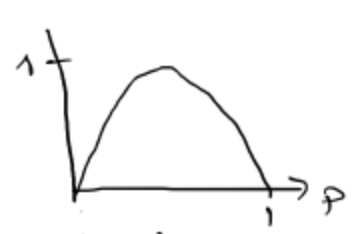
\includegraphics[width=.7\linewidth]{SCR-20240305-qtnt.png}
    Compression factor for different values of \(p\).
    As \(p\) approaches 0.5 from either side,
    we can compress the message less and less,
    since there is more entropy we need to encode.

    \subsection{Shannon's Noiseless Coding Theorem:}
    For a given message,
    we only need \(N H(p)\) bits to encode it (definition of \(H(p)\) above)

    \textbf{Example:}
    Let us have an alphabet A, B, C, D
    with probabilities of \(1/2, 1/4, 1/8, 1/8\) respectively.
    Entropy is \(H = -(1/2 \log 1/2 + 1/4 \log 1/4 \dots) = 7/4\text{ bits}\)
    Therefore, a message \(N\) characters long can be encoded in \(7/4 \cdot N\) bits.

    \subsection{Shannon's Noisy Coding Theorem:}
    On average, we need at least \(\frac{N_0}{1-H(q)}\)
    bits to encode one of \(2^{N_0}\) equally probable messages
    (\(N_0\) is the original message length)
    where \(H(q) = -[q \log q + (1-q) \log (1-q)]\)
    is the entropy associated with single bit error q.

    \textbf{Efficient Coding:}
    Plot \(N/N_0 - 1\) vs \(q\) to see when overhead becomes too ``large''

    \textbf{Huffman Coding}
    \begin{enumerate}
        \item Sort the probabilities
        \item Combine the two lowest probabilities into a tree,
              storing characters as branches and the sum of their probabilities as the root
        \item Repeat until all probabilities are combined, and we reach a probability of 1
        \item Set 0/1 to left/right (either pairing), and traverse the tree to find the encoding
    \end{enumerate}

    \section{Dirac Notation}
    \(\bra{\Psi} \Longleftrightarrow \ket{\psi}^\dagger\)

    \begin{tabular}{@{}lc@{}}\toprule
        Ket                        & Matrix                                                         \\ \midrule
        \(\ket{0}\) or \(\ket{H}\) & \(\begin{bmatrix} 1 \\ 0 \end{bmatrix}\)                       \\
        \(\ket{1}\) or \(\ket{V}\) & \(\begin{bmatrix} 0 \\ 1 \end{bmatrix}\)                       \\
        Diagonal Up                & \(\frac{1}{\sqrt{2}}\begin{bmatrix} 1 \\ 1 \end{bmatrix}\)     \\
        Diagonal Down              & \(\frac{1}{\sqrt{2}}\begin{bmatrix} 1 \\ -1 \end{bmatrix}\)    \\
        Left Circular              & \(\frac{1}{\sqrt{2}}\begin{bmatrix} 1 \\ i \end{bmatrix}\)     \\
        Right Circular             & \(\frac{1}{\sqrt{2}}\begin{bmatrix} 1 \\ -i \end{bmatrix}\)    \\
        \( \theta \)               & \(\begin{bmatrix} \cos \theta \\ \sin \theta \end{bmatrix}\)   \\
        \(\pi / 2 + \theta \)      & \(\begin{bmatrix} - \sin \theta \\ \cos \theta \end{bmatrix}\) \\
        \bottomrule
    \end{tabular}

    \includegraphics[width=.7\linewidth]{Bloch\_sphere.svg.png}

    \(\ket{\Psi} = \cos\frac{\theta}{2}\ket{0}+e^{i \phi}\sin\frac{\theta}{2}\ket{1}\)

    \begin{multicols*}{2}
        \(+x = \frac{1}{\sqrt{2}}(\ket{0}+\ket{1})\)
        \(-x = \frac{1}{\sqrt{2}}(\ket{0}-\ket{1})\)
        \(+y = \frac{1}{\sqrt{2}}(\ket{0}+i\ket{1})\)
        \(-y = \frac{1}{\sqrt{2}}(\ket{0}-i\ket{1})\)
    \end{multicols*}

    \subsection{Change of basis}
    Let \(\theta\) be a rotation of basis vectors,
    counterclockwise.

    \(\ket{x} = \cos\theta\ket{x'} - \sin\theta\ket{y'}\)
    and
    \(\ket{y} = \sin\theta\ket{x'} + \cos\theta\ket{y'}\)

    where \(\ket{x'}\) and \(\ket{y'}\) are the new basis vectors.

    \subsection{Outer Product}
    Given that
    \(\ket{\psi} = \)
    \(\ket{\psi}\bra{\phi} = \begin{bmatrix} \psi_1\phi_1 & \psi_1\phi_2 \\ \psi_2\phi_1 & \psi_2\phi_2 \end{bmatrix}\)

    \subsection{Quantum State Tomography}
    \begin{itemize}
        \item Set a set of observables to uniquely determine a state.
              For a single qubit, we can use the Pauli operators.
        \item Prepare many copies of the state
        \item Measure the observables in states $\{H, V\}, \{+45, -45\}, \{LCP, RCP\}$
        \item Decompose state as $\ket{\psi} = r_H \ket{H} + r_V e^{i \phi} \ket{V}$
              where $\phi = \phi_V - \phi_H$
        \item Procedure
              \begin{enumerate}
                  \item Perform measurement in \{H, V\} basis - Probability of detecting H is $r_H^2$, so $r_H = \sqrt{Pr_H}, r_v = \sqrt{1 - Pr_H}$
                  \item $\cos \phi = \frac{Pr_{+45} - 1/2}{\sqrt{(1 - Pr_H)(Pr_H)}}$
                  \item $\sin_\phi = \frac{1/2 - Pr_{RCP}}{\sqrt{(1 - Pr_H)(Pr_H)}}$
              \end{enumerate}
    \end{itemize}

    \section{Operators}
    Operators produce another ket

    \subsection{Spectral Decomposition}
    Operator $A$ can be decomposed
    $
        \hat{A} = \sum_i a_i \ket{a_i} \bra{a_i}
    $

    \subsection{Observable}
    Is an operator, likely one of the Pauli operators.
    The measured results when observing in this ``direction'' will be one of its eigenvalues.

    \textbf{Mean value of an observable}
    Measuring an observable
    \(\hat{V} = \sum_i v_i \ket{v_i}\bra{v_i}\)
    in the state \(\ket{\Psi}\)

    Obtains result \(v_i\) with probability
    \(p(v_i) = |\braket{v_i|\Psi}|^2\)

    Repeating measurement many times obtains \textbf{expectation value}
    \(\braket{V}=\sum_i P_i v_i = \sum_i |\braket{v_i|\Psi}|^2 v_i\)
    \(\braket{V}_\Psi = \braket{\Psi|\hat{V}|\Psi}\)

    \subsection{Uncertainty}
    Variance is
    \(
    \Delta V^2
    = \braket{\Psi|(\hat{V}-\braket{\Psi|\hat{V}|\Psi})^2|\Psi}
    \)
    \(
    \Delta V^2
    = \braket{\Psi|\hat{V}^2|\Psi} - \braket{\Psi|\hat{V}|\Psi}^2
    = \braket{\hat{V}^2}-\braket{\hat{V}}^2
    \)

    \subsection{Heisenberg Uncertainty Principle}
    \(\Delta x \Delta p \geq \frac{1}{2} |\braket{\psi | [\hat{A}, \hat{B}]| \psi}|\)
    (e.g. for \([\hat{x}, \hat{p}] = i \hbar\) we find \(\Delta x \Delta p \geq \frac{\hbar}{2}\))

    \subsection{Pauli Operators}

    \begin{tabular}{@{}l@{}} \toprule
        \(\hat{\sigma}_x
        = \begin{pmatrix}
              0 & 1 \\
              1 & 0
          \end{pmatrix}
        = \ket{0}\bra{1}+\ket{1}\bra{0}\)    \\
        \quad Eigenvectors: \(
        \begin{pmatrix}1\\0\end{pmatrix},
        \begin{pmatrix}0\\1\end{pmatrix}
        \)                                   \\
        \(\hat{\sigma}_y
        = \begin{pmatrix}
              0 & -i \\
              i & 0
          \end{pmatrix}
        = i(\ket{1}\bra{0}-\ket{0}\bra{1})\) \\
        \quad Eigenvectors: \(
        \frac{1}{\sqrt{2}}\begin{pmatrix}1\\i\end{pmatrix},
        \frac{1}{\sqrt{2}}\begin{pmatrix}1\\-i\end{pmatrix}
        \)                                   \\
        \(\hat{\sigma}_z
        = \begin{pmatrix}
              1 & 0  \\
              0 & -1
          \end{pmatrix}
        = \ket{0}\bra{0}-\ket{1}\bra{1}\)    \\
        \quad Eigenvectors: \(
        \frac{1}{\sqrt{2}}\begin{pmatrix}1\\1\end{pmatrix},
        \frac{1}{\sqrt{2}}\begin{pmatrix}1\\-1\end{pmatrix}
        \)                                   \\
        \(\hat{I}
        = \begin{pmatrix}
              1 & 0 \\
              0 & 1
          \end{pmatrix}
        = \ket{0}\bra{0}+\ket{1}\bra{1}\)    \\
        \quad Eigenvectors: \(
        \begin{pmatrix}0\\1\end{pmatrix},
        \begin{pmatrix}1\\0\end{pmatrix}
        \)                                   \\
        \bottomrule
    \end{tabular}

    (All have respective eigenvalues of +1 and -1)

    \subsubsection{Commutaton Relations}
    \begin{multicols*}{2}
        \begin{align*}
            [\hat{\sigma}_x, \hat{\sigma}_y] & = 2i\hat{\sigma}_z \\
            [\hat{\sigma}_y, \hat{\sigma}_z] & = 2i\hat{\sigma}_x \\
            [\hat{\sigma}_z, \hat{\sigma}_x] & = 2i\hat{\sigma}_y
        \end{align*}
        \begin{align*}
            \{\hat{\sigma}_x, \hat{\sigma}_y\} & = 0 \\
            \{\hat{\sigma}_y, \hat{\sigma}_z\} & = 0 \\
            \{\hat{\sigma}_z, \hat{\sigma}_x\} & = 0
        \end{align*}
    \end{multicols*}
    \([\hat{\sigma}_a, \hat{\sigma}_b]=2 i \epsilon_{abc} \hat{\sigma}_c\)

    For direction \(\vec{n}\),
    \(
    \vec{n} \cdot \vec{\hat{\sigma}}
    = n_x \hat{\sigma}_x
    + n_y \hat(\sigma)_y
    + n_z \hat{\sigma}_z
    \)

    For any operator,
    \begin{align*}
        \hat{H} & = \begin{pmatrix}
                        a      & c - id \\
                        c + id & b
                    \end{pmatrix}                                                                                 \\
                & = \frac{a+b}{2}\hat{\mathbb{I}} + \frac{a-b}{2}\hat{\sigma}_z + c\hat{\sigma}_x + d\hat{\sigma}_y
    \end{align*}

    \section{Tensor Products}
    Given that \(\ket{\psi} = \begin{pmatrix} a \\ b \end{pmatrix}\)
    and \(\ket{\phi} = \begin{pmatrix} c \\ d \end{pmatrix}\)
    \[
        \ket{\psi} \otimes \ket{\phi}
        = \begin{pmatrix}
            a\begin{pmatrix} c \\ d \end{pmatrix} \\
            b\begin{pmatrix} c \\ d \end{pmatrix}
        \end{pmatrix}
        = \begin{pmatrix}
            ac \\
            ad \\
            bc \\
            bd
        \end{pmatrix}
    \]

    For operators,
    \begin{align*}
        \hat{A} \otimes \hat{B}
         & = \begin{pmatrix}
                 a & b \\
                 c & d
             \end{pmatrix}
        \otimes
        \begin{pmatrix}
            \alpha & \beta  \\
            \gamma & \delta
        \end{pmatrix}                            \\
         & = \begin{pmatrix}
                 a\begin{pmatrix}
                 \alpha & \beta  \\
                 \gamma & \delta
             \end{pmatrix} &
                 b\begin{pmatrix}
                 \alpha & \beta  \\
                 \gamma & \delta
             \end{pmatrix} \\
                 c\begin{pmatrix}
                 \alpha & \beta  \\
                 \gamma & \delta
             \end{pmatrix} &
                 d\begin{pmatrix}
                 \alpha & \beta  \\
                 \gamma & \delta
             \end{pmatrix}
             \end{pmatrix}          \\
         & = \begin{pmatrix}
                 a\alpha & a\beta  & b\alpha & b\beta  \\
                 a\gamma & a\delta & b\gamma & b\delta \\
                 c\alpha & c\beta  & d\alpha & d\beta  \\
                 c\gamma & c\delta & d\gamma & d\delta
             \end{pmatrix}
    \end{align*}

    \subsection{Properties}
    Not commutative.
    Distributive:
    \(\ket{\psi}\otimes(\ket{\phi}+\ket{\varphi}) = \ket{\psi}\otimes\ket{\phi}+\ket{\psi}\otimes\ket{\varphi}\)
    \(\hat{A}\otimes(\hat{B}+\hat{C}) = \hat{A}\otimes\hat{B}+\hat{A}\otimes\hat{C}\)

    Operators can act on one photon and not the other:
    Eg, let
    \[
        \sigma_A^x
        = \begin{pmatrix}
            0 & 0 & 1 & 0 \\
            0 & 0 & 0 & 1 \\
            1 & 0 & 0 & 0 \\
            0 & 1 & 0 & 0
        \end{pmatrix}
    \]
    thus,
    \begin{align*}
        \sigma_A^x \ket{HH}
         & = \sigma_A^x \otimes \mathcal{I} (\ket{H}_A \otimes \ket{H}_B) \\
         & = (\sigma_A^x \ket{H}_A) \otimes (\mathcal{I} \ket{H}_B)       \\
         & = \ket{V}_A \otimes \ket{H}_B                                  \\
         & = \ket{VH}
    \end{align*}
    or
    \[
        \begin{pmatrix}
            0 & 0 & 1 & 0 \\
            0 & 0 & 0 & 1 \\
            1 & 0 & 0 & 0 \\
            0 & 1 & 0 & 0
        \end{pmatrix}
        \begin{pmatrix}
            1 \\
            0 \\
            0 \\
            0
        \end{pmatrix}
        =
        \begin{pmatrix}
            0 \\
            0 \\
            1 \\
            0
        \end{pmatrix}
    \]

    \section{Classical Cryptography}
    \textbf{Criterion for Perfect Secrecy}
    Let \(\{p_i\}\) be the set of possible plaintexts,
    and \(\{c_j\}\) be the set of possible ciphertexts.
    \(
    P(p_i | C_j) = P(p_i) \forall i, j
    \)
    (discovering a ciphertext provides no information about the plaintext)

    % TODO: add classical cryptosystem examples

    \section{Quantum Cryptography}
    Based on no-cloning theorem (cannot copy an unknown quantum state)

    \subsection{BB84 (Quantum Key Distribution)}
    \begin{enumerate}
        \item Alice sends a random sequence of bits, randomly encoded in either H/V or +45/-45 basis, to Bob
        \item Bob measures each qubit in a random basis
        \item Alice and Bob compare bases used
        \item Alice and Bob discard qubits measured in different bases
        \item Alice and Bob compare a subset of their qubits to check for eavesdropping
        \item Alice and Bob use the remaining qubits as a shared key
        \item Alice and Bob use the shared key to encrypt and decrypt messages
    \end{enumerate}
    Errors in the key indicate eavesdropping
    (probability that Eve does not cause an error is \((3/4)^N\),
    where \(N\) is the number of qubits tested)

    \subsection{B92 Protocol}
    Non-orthogonal bases, eg \(\ket{0}, \ket{1}\) and \(\ket{0'}, \ket{1'}\)
    Alice prepares states in \(\ket{0}, \ket{1'}\),
    associating them with 0 and 1, and sends them to Bob.

    Bob measures in the two basis randomly.
    If he receives a \(\ket{0}\), he discards it,
    as it could have been prepared as \(\ket{0}\) or \(\ket{1'}\),
    but if he receives a \(\ket{1}\), he knows it was prepared as \(\ket{1'}\).
    Same for \(\ket{0'}, \ket{1'}\)

    \textbf{Advantages:} Only needs 2 states and 2 basis, unconditionally secure in a lossless channel,
    does not make use of entanglement.

    \subsection{Ekert's Entangled State Protocol}
    \begin{itemize}
        \item $\ket \Psi^-$ kets, keep qubit A, send b
        \item Generated key is anti-correlated, Bob flips his measured result
    \end{itemize}

    \section{Entanglement}
    \subsection{Bell states}
    \begin{align*}
        \ket{\Psi^+} = \frac{1}{\sqrt{2}} (\ket{HV} + \ket{VH}) \\
        \ket{\Psi^-} = \frac{1}{\sqrt{2}} (\ket{HV} - \ket{VH}) \\
        \ket{\Phi^+} = \frac{1}{\sqrt{2}} (\ket{HH} + \ket{VV}) \\
        \ket{\Phi^-} = \frac{1}{\sqrt{2}} (\ket{HH} - \ket{VV})
    \end{align*}
    \(\Psi^-\) is isotropic (it remains the same no matter which axes we choose to measure it along)
    By decomposing it into \(\theta\) basis, we can show that
    \(\Psi^- = \frac{1}{\sqrt{2}}(\ket{HV} - \ket{VH}) = \frac{1}{\sqrt{2}}(\ket{\theta, \theta + \pi/2} - \ket{\theta + \pi/2, \theta})\)

    \subsection{Density matrix formalism}
    \textbf{Density Operator:}
    \(\hat{\rho} = \sum_n p_n \ket{\psi_n}\bra{\psi_n}\)
    \(\sum_i p_i = 1\)
    We can treat this as a ``sum of probabilities'',
    where \(p_i\) is the probability of a given state \(\ket{\psi_i}\) appearing.
    The states for \(\psi_n\) need not be orthogonal.

    We can rewrite it as
    \(\hat \rho = \sum_m p_m \ket p_m \bra p_m \)

    \textbf{Measurement / Expectation Value / Generalized Born Rule}
    Measuring using a Hermitian operator $M = \sum_i m_i \ket{m_i} \bra{m_i}$
    results in one of its eigenvalues $m_i$.
    The probability of obtaining a nondegenerate eigenvalue $m_i$ is
    $p(m_i) = Tr[\rho \Pi_i]$,
    where $\Pi_i \equiv \ket m_i \bra m_i$.
    If eigenvalues are degenerate, with value $m$,
    the probability of finding that value is $\sum_i Tr[\rho \Pi_i]$,
    where the sum is over the values of $i$ where $m_i = m$.

    \textbf{Measuring GHZ State}
    To measure only the first two qubits, measure all 3 qubits twice,
    performing 2 measurements for the last qubit.


    \textbf{Purity:}
    \(Tr(\hat{\rho}^2) = \sum_m \rho_m^2\) is the purity of a state
    Essentially how separable / correlated the two states are.

    \subsubsection{Properties}
    If $\hat{\rho}$ is diagonal and more than a single diagonal element is not 0,
    then it must be a mixed state.
    Measurements reduce a quantum state to a statistical mixture.
    $Tr(\ket 0 \bra 0) = Tr(\ket 1 \bra 1) = 1$
    $Tr(\ket 0 \bra 1) = Tr(\ket 1 \bra 0) = 0$

    \subsection{Reduced density matrices}
    Given a state,
    \[
        \ket{\psi_{AB}}
    \]
    The density operator for this state can be separated
    \[
        \rho_{AB} = \ket{\psi_{AB}}\bra{\psi_{AB}}
        = \ket{\psi_A}\bra{\psi_A} \otimes \ket{\psi_B}\bra{\psi_B}
    \]
    And satisfies the equality \(\operatorname{Tr} \rho_{AB}^2 = 1\),
    since it is coherent.
    Therefore,
    \begin{align*}
        \operatorname{Tr}_B \rho_{AB} = \rho_A & \quad \operatorname{Tr}_A \rho_{AB} = \rho_B \\
        \rho_A = \ket{\psi_A}\bra{\psi_A}      & \quad \rho_B = \ket{\psi_B}\bra{\psi_B}
    \end{align*}

    \subsection{Von Neumann entropy}
    \(S = -Tr(\rho \ln \rho) = -\sum_i p_i \ln p_i\)
    where $p_i^A$ are diagonal elements in $\rho_A$

    \section{EPR Paradox}
    Say Alice and Bob share state \(\ket{\Psi^-} = \frac{1}{\sqrt{2}} (\ket{0} - \ket{1})\)
    \begin{itemize}
        \item If A is measured in Z, then B measures opposite Z
        \item Same for X measurement on A
        \item Predict either Z or X of qubit B by performing one or the other on A.
        \item If our choice does not disturb B, then the values for X and Z must exist simultaneously, so there must be hidden variables
        \item TL;DR, believed there was a theory as correct as QM that could deterministically predict results of Bob's measurements
    \end{itemize}

    \subsection{Local Realism}
    Local realism is the idea that the properties of a system are determined by the properties of the system's parts.
    AKA, no spooky action at a distance.

    \subsection{Bell's Inequality:}
    Front-panel explanation:
    \begin{itemize}
        \item Source sends out pairs of particles, each appratus has buttons marked M, N,
              Alice and Bob randomly measure in these states w/o communication.
        \item Each apparatus displayes a readout depending on results.
        \item Alice and Bob record their events.
        \item We assert that $\sum{M_A M_B N_A N_B} P(M_A, M_B, N_A, N_B) = 1$,
              such that all 4 quantities have well-defined values (say in a hidden variable),
              even though only 2 of them are displayed. (Locality)
        \item From this, we assert that $|< M_A M_B - M_A N_B + N_A M_B + N_A N_B >| \leq 2$ if locality holds.
        \item However, each expectation value is actually $\pm 1/\sqrt{2}$, leading to a final value of $<S> = -2 \sqrt{2}$.
        \item Contradiction!
    \end{itemize}

    \subsubsection{Loop Holes}
    \textbf{Locality loophole}
    If Alice and Bob are close, then information could be transmitted, and thus measurements are no longer ``local''

    \textbf{Detection loophole}
    If one or more photons are lost, then the situation is no longer consistent with the ``front panel'' described.
    Taking into account only the events that do occur doesn't refute local realism.
    e.g. a hidden variable that decides if it should appear ``invisible'',
    causing it to not have values for M and N at the same time

    \subsubsection{GHZ State}
    GHZ State can also show non-locality:
    \begin{itemize}
        \item 3 observers, each with a Bell apparatus,
              but buttons are for $\hat\sigma_x$ and $\hat\sigma_y$ measurements.
        \item Source sends out 3 particles at a time
        \item Note that whenever 2 are $\hat\sigma_y$ and 1 is $\hat\sigma_x$,
              result is -1.
        \item Local realism predicts that $\sigma_{xA}\sigma_{xB}\sigma_{xC} = -1$
        \item However, $\sigma_{xA}\sigma_{xB}\sigma_{xC} \ket{GHZ} = +\ket{GHZ}$, with an eigenvalue of +1.
              Contradiction.
    \end{itemize}

    \subsection{CHSH Game:}
    We can construct a game to test Bell's inequality.
    Alice and Bob each have a bit, and they can choose to measure it in one of two bases.
    They win if the XOR of their bits is 0.

    Using deterministic strategies, the maximum win rate is 75\%.

    However, using entangled particles, we can achieve a win rate of 85\%,
    violating Bell's inequality.

    \subsection{Quantum Socks}
    \begin{itemize}
        \item Generate $\ket \psi^-$
    \end{itemize}

    \section{Quantum Dense Coding}
    \begin{itemize}
        \item Start with shared qubit $\ket{\Psi^-}$
        \item Alice applies one of $\{\hat I, \hat\sigma_x, \hat\sigma_y, \hat\sigma_z\}$ to just her qubit,
              producing the following conversions:
              $\hat I \otimes \hat I \ket{\Psi^-} = \ket{\Psi^-}$
              $\hat \sigma_x \otimes \hat I \ket{\Psi^-} = -\ket{\Phi^-}$
              $\hat \sigma_y \otimes \hat I \ket{\Psi^-} = i\ket{\Phi^+}$
              $\hat \sigma_z \otimes \hat I \ket{\Psi^-} = \ket{\Psi^+}$
              (we ignore global phases $-$ and $i$)
        \item Alice then sends single qubit to Bob
        \item Bob then measures in Bell-state basis, with a CNOT with 1 as control and 2 as target,
              and a Hadamard gate on 1. This maps
              $\ket{\Psi^-} \to \ket{11}$,
              $\ket{\Psi^+} \to \ket{01}$,
              $\ket{\Phi^-} \to \ket{10}$,
              $\ket{\Phi^+} \to \ket{00}$.
        \item Neither Bob nor Alice can recover the encoded information alone,
              instead the information resides in correlations between two qubits, and is non-local.
    \end{itemize}

    \section{Quantum Teleportation}
    \begin{itemize}
        \item Transfers unknown quantum state between 2 locations
        \item Uses classical communications channel
        \item Original state is destroyed
    \end{itemize}
    \subsection{Procedure}
    \begin{itemize}
        \item Input state of $\ket{\chi} = \alpha \ket{H} + \beta \ket{V}$ in Hilbert space $V_1$
        \item Alice and Bob share entangled state $\ket{\Psi^-}$ in Hilbert space $V_2 \otimes V_3$
        \item Alice measures in $V_1 \otimes V_2$ space in the bell basis
    \end{itemize}

    \begin{tabular}{@{}llll@{}} \toprule
        Alice    & Prob & Bob                                 & Op                         \\ \midrule
        $\Phi^+$ & 1/4  & $-\beta \ket{H} + \alpha \ket{V}$   & $\rho_z \rho_x = i \rho_y$ \\
        $\Phi^-$ & 1/4  & $\beta \ket{H} + \alpha \ket{V}$    & $\rho_x$                   \\
        $\Psi^+$ & 1/4  & $-\alpha \ket{H} + \beta \ket{V}$   & $\rho_z$                   \\
        $\Psi^-$ & 1/4  & $-(\alpha \ket{H} + \beta \ket{V})$ & none                       \\
        \bottomrule
    \end{tabular}

    \section{Quantum Repeater}
    \begin{itemize}
        \item Entangle each link's cells, not very likely to succeed but each link can be retried until connection is made
        \item Entangle link ends (that are very close and will very likely succeed) to form final long link
    \end{itemize}
    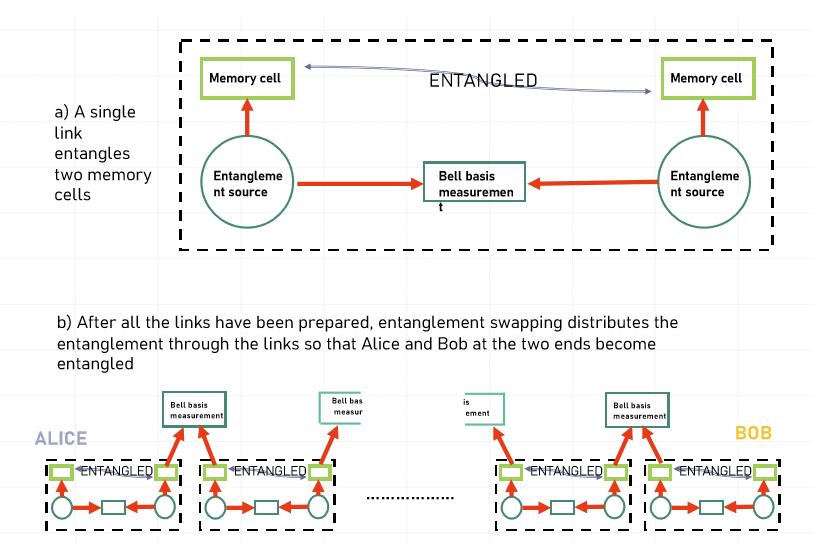
\includegraphics[width=\linewidth]{Quantum Repeater.png}

    \section{Quantum Gates}
    \subsection{Properties}
    \begin{itemize}
        \item Can only perform unitary operations
              \begin{itemize}
                  \item Due to all quantum operations being unitary, follows from Schrodinger's equation
                  \item If it were not unitary, we would be discarding data which is a ``measurement''
              \end{itemize}
        \item Any controlled-unitary gate can be made from CNOT and single qubit gates.
    \end{itemize}

    \subsection{Necessary Conditions}
    \begin{itemize}
        \item Well-defined, extendible qubit array that is stable
        \item Ability to prepare qubit array in suitable starting state, eg all $\ket{0}$
        \item Good isolation from environment (long coherence times)
        \item Ability to perform universal set of gate operations (e.g. single-qubit rotations, CNOT between any pair of qubits)
        \item Ability to perform close to ideal von Neumann measurements on each of the qubits
    \end{itemize}

    % TODO: maybe add other approaches

    \subsection{Unitary}
    Unitary if $A^\dagger A = \mathbb{I}$,
    where $\dagger$ represents conjugate transform (Hermitian Conjugate).

    \subsection{Common Gates}
    \textbf{Hadamard gate:}
    \(\hat{H} = \frac{1}{\sqrt{2}} \begin{pmatrix}
        1 & 1  \\
        1 & -1
    \end{pmatrix}
    = \frac{1}{\sqrt{2}} (\hat{\sigma_z} + \hat{\sigma_x})\)
    \textbf{Rotation operator:}
    \(\hat{R}(\vec{n}, \theta) = e^{-i \theta \vec{n} \cdot \vec{\hat{J}}}\)
    Where \(\vec{\hat{J}}\) is the angular momentum operator,
    and \(\vec{n} = (\sin\theta\cos\phi, \sin\theta\sin\phi, \cos\theta)\)
    is a unit vector.

    For spin-1/2, \(\vec{\hat{J}} = \frac{1}{2}\vec{\hat{\sigma}}\)

    \subsection{2-qubit Quantum Gates}
    $\ket{00} \Leftrightarrow \begin{pmatrix}1\\0\\0\\0\end{pmatrix}$
    $\ket{01} \Leftrightarrow \begin{pmatrix}0\\1\\0\\0\end{pmatrix}$
    $\ket{10} \Leftrightarrow \begin{pmatrix}0\\0\\1\\0\end{pmatrix}$
    $\ket{11} \Leftrightarrow \begin{pmatrix}0\\0\\0\\1\end{pmatrix}$

    Matrix is 4 by 4, selected column(s) can be treated as ``inputs'',
    row values in said column(s) are ``outputs''.

    \section{Quantum Algorithms}
    \subsection{Deutsch-Joza Algorithm}
    Determine whether an unknown selection from 4 1-bit functions is constant or balanced.

    Classical algorithm requires 2 evaluations for f(0) and f(1)

    Quantum algorithm evaluates both f(0) and f(1) at the same time:
    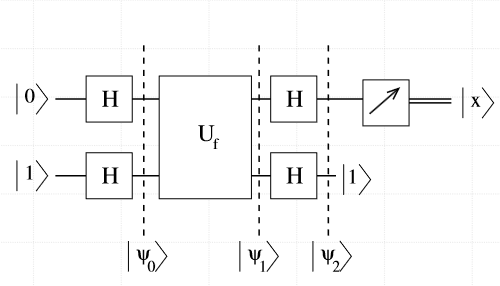
\includegraphics[width=\linewidth]{DJ Algo.png}
    If $f(0) = f(1) = \pm \ket{0}$, else $f(0) = \pm \ket{1} \neq f(1)$.

    \subsubsection{N qubit extension}
    Classical has $O(2^N)$ time complexity, QM has constant time (single Oracle use).

    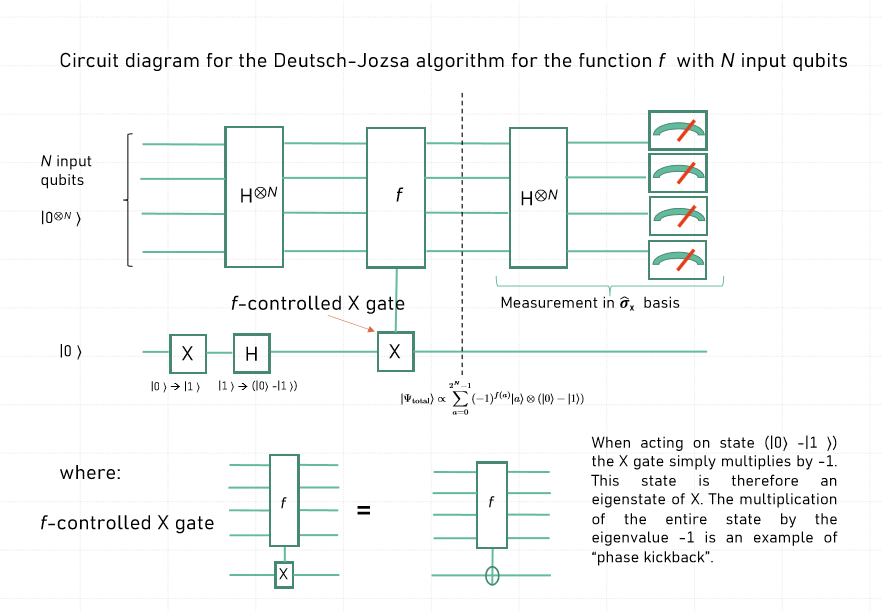
\includegraphics[width=\linewidth]{DJ Algo Extension.png}

    If $f$ is constant, amplitude is either +1 or -1, so measurement must give all 0s.
    Otherwise, it will not be all 0s.

    \subsection{Bernstein-Vazirani Algorithm}
    Given a function $f(x) = a \cdot x$, find $a$.

    Classically, we would need to do $n$ queries, one for each bit.

    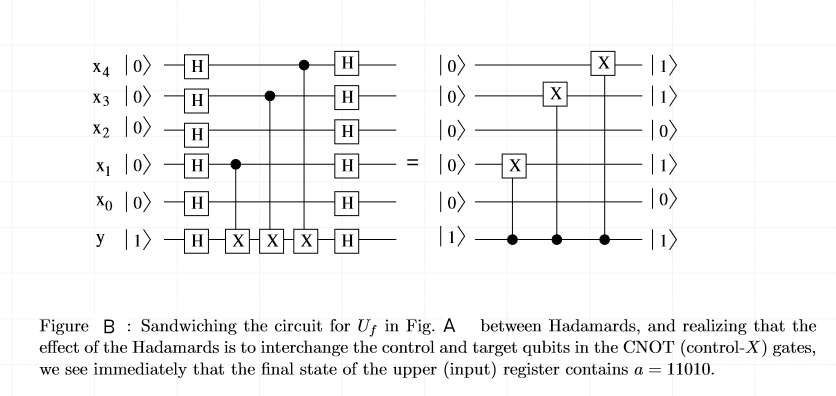
\includegraphics[width=\linewidth]{BV Algo.png}

    Using QM, we can get the positisons in $a$ that are 1 using one query.

    \subsection{Simon's Algorithm}
    Given a black-box function that has the property $f(x \oplus a) = f(x)$, find $a$.
    Since $x \oplus a \oplus a = x$, $f(x) = f(x \oplus a) = f(x \oplus a \oplus a)$,
    therefore $f(x)$ is periodic with period $a$ under bitwise mod 2 addition.

    Classically, we evaluate functions on different inputs until we find a repetition,
    and then compare $m(m-1)/2$ pairs.
    For a good chance of success, number of pairs must be close to $2^n$,
    so $m$ is to the order of $2^{n/2}$.

    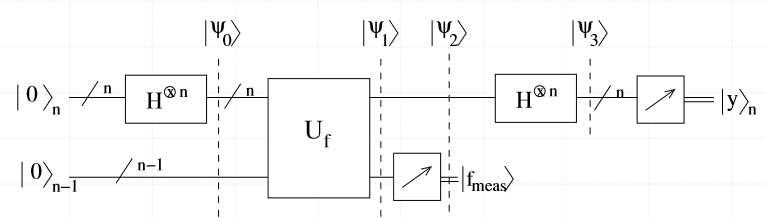
\includegraphics[width=\linewidth]{Simon's Algo.png}

    Using the multiple measurements performed at $y$, the bit indicies with 1s form a linear equation,
    that equal 0. Combining multiple of these measurements, we can build a valid solution.

    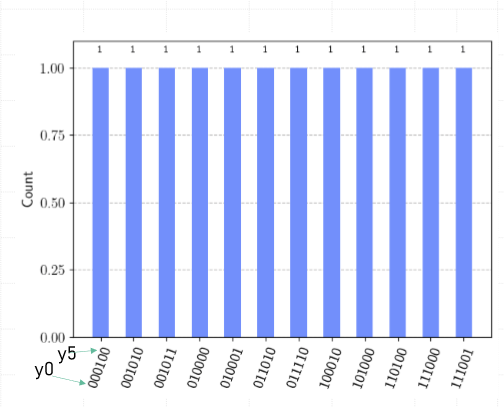
\includegraphics[width=\linewidth]{Simon's Algo Results.png}
    e.g. in this case,
    $a3 = 0$, $a2 + a4 = 0$, $a2 + a4 + a5 = 0$... and we find that $a = 010101$.

    \subsection{Shor's Algorithm}
    Given an integer $N$, what are its prime factors?

    Classical algorithm: ``General number field sieve'',
    runs in exponential time w.r.t. input length.

    Theory
    \begin{itemize}
        \item Let $N$ be the product of two prime numbers $p$ and $q$.
              Thus, the sequence $m \mod N, m^2 \mod N, m^3 \mod N, \dots$ will repeat with a period
              that is a perfect divisor of $(p-1)(q-1)$
        \item Use Quantum Fourier Transform to find the period of this sequence
    \end{itemize}

    Algorithm
    \begin{enumerate}
        \item Pick a random integer $a$ with no common factors with $N$.
        \item Calculate $a, a^2, a^4 \dots, a^{2^n} \pmod N$, where $2^n > N^2$
        \item Perform modular exponentiation for all $x$, a.k.a $a^x = \prod_{j=0}^{n-1} (a^{2^j})^{x_j}$
              (algorithm below up to $\Psi_1$)
        \item QFT to extract the period of probabilities from upper register
        \item If successful, we find $y$ within $1/2$ of $2^n m/r$, and thus $|y/2^n - m/r| < 1/2^{n+1}$.
        \item Thus, $m/r$ is one of partial sums of continued fraction expansion of $y/2^n$
    \end{enumerate}

    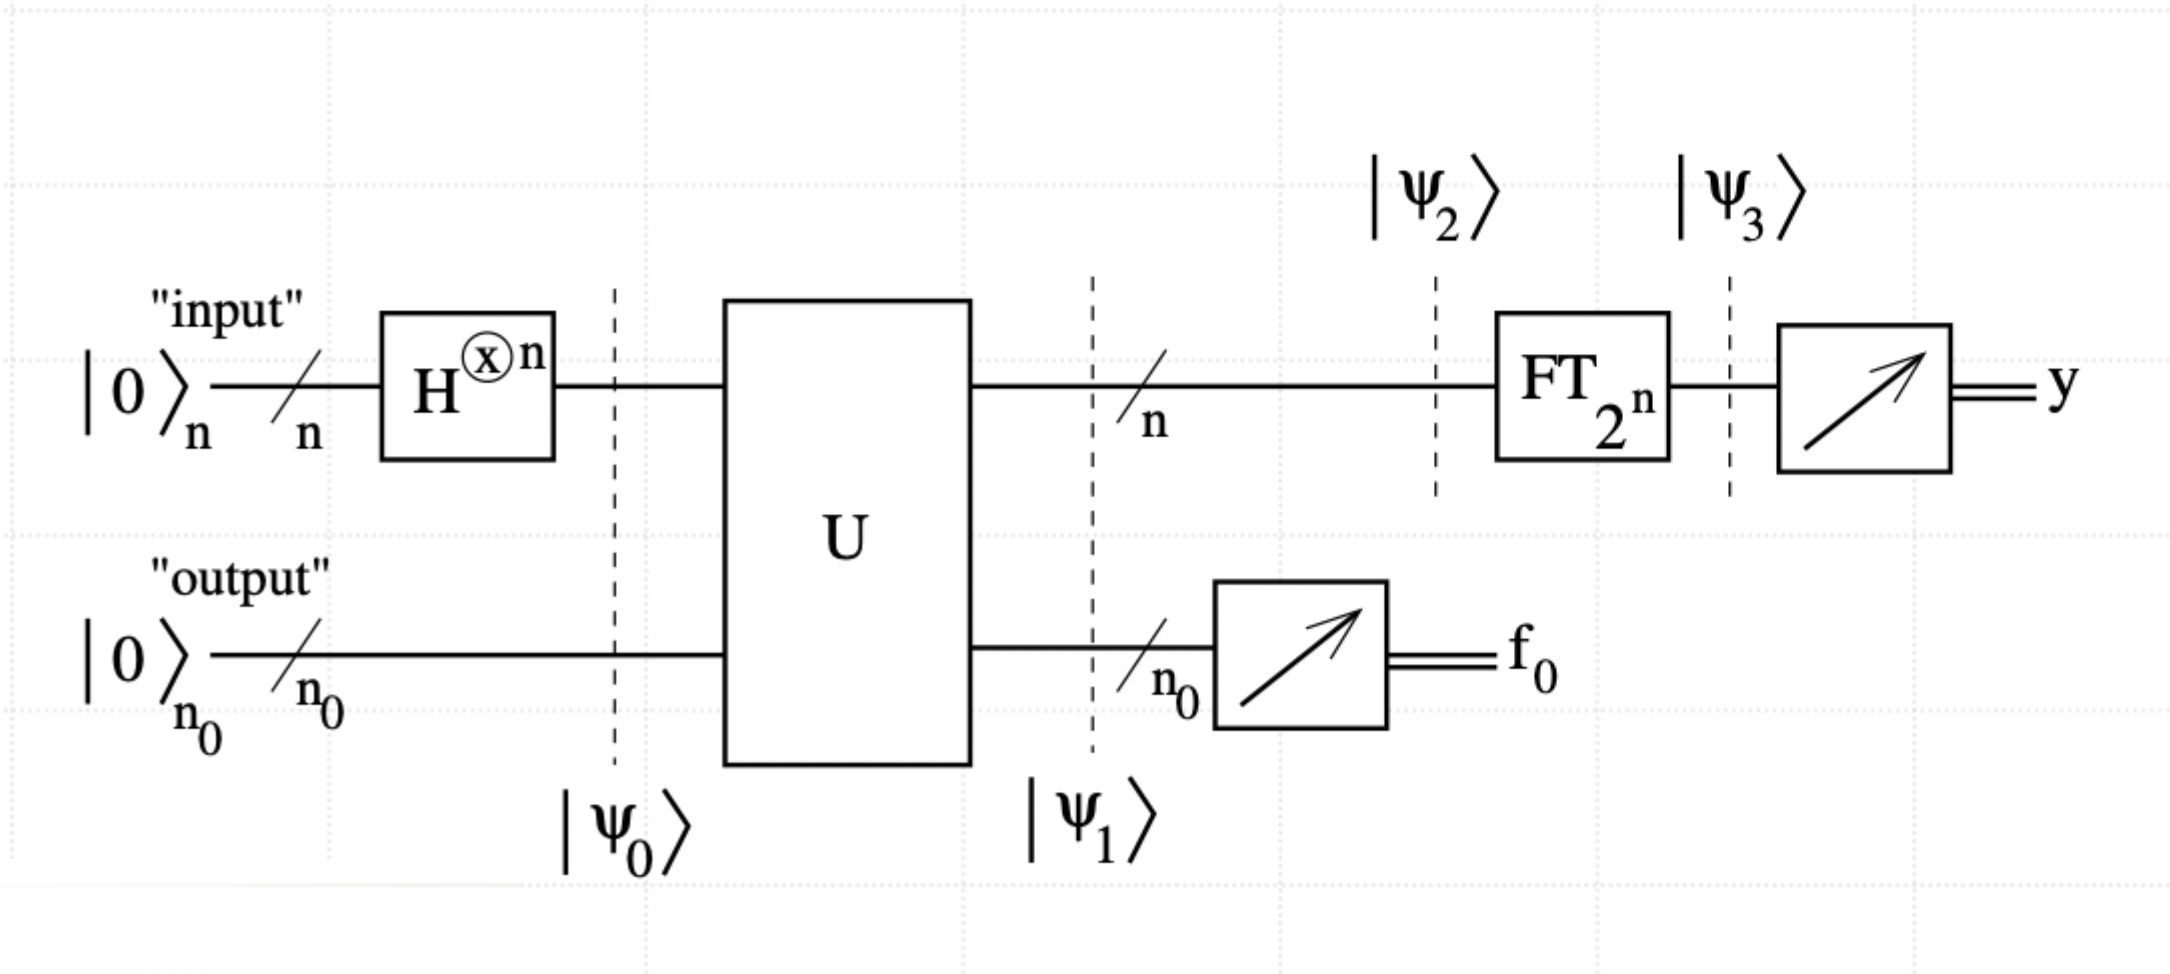
\includegraphics[width=\linewidth]{Shor.png}

    \section{Coherent Superposition}
    \begin{itemize}
        \item Must be a well-defined phase between pieces in superposition
        \item e.g. there can eventually be interference between pieces
        \item If the phase is random, no interference exists,
              and we return to classical addition of probabilities
        \item Coherent sum of amplitudes: $1/2 |\alpha + \beta|^2$
        \item Incoherent average over probabilities: $1/2 (|\alpha|^2 + |\beta|^2)$
    \end{itemize}

    \section{Quantum Error Correction}
    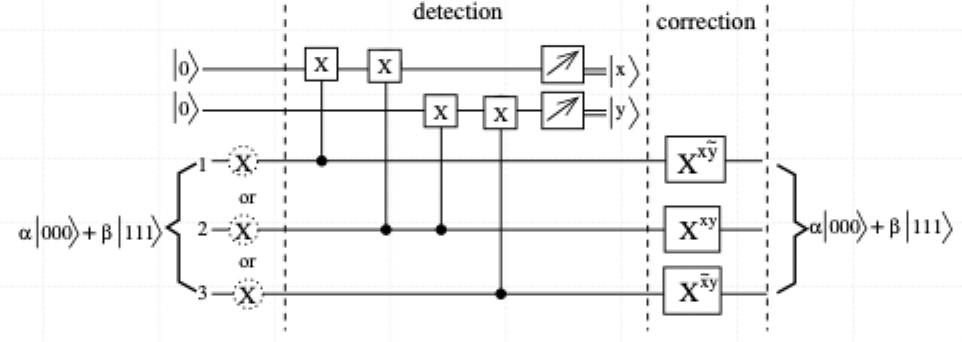
\includegraphics[width=\linewidth]{Ancilla Quantum Error Correction.png}
    Measurement of Ancilla identifies and collapses the error,
    and applying the appropriate operator corrects the error.

    \subsection{Stabilizers}
    \begin{itemize}
        \item Square to 1 (so eigenvalues are $\pm 1$)
        \item Mutually commute, so have same eigenstates
        \item Syndromes are eigenstates
        \item Uncorrupted syndrome has eigenvalue +1 for all stabilizers
        \item Set of $\pm 1$ eigenvalues of stabilizers uniquely specifies syndrome
    \end{itemize}

    \subsection{Phase Flip Errors}

    Given errors of the type
    $\ket \psi = \alpha \ket 0 + \beta \ket 1 \to \alpha \ket 0 - \beta \ket 1$

    \begin{itemize}
        \item Correct by transforming to +- basis of X operator
        \item Use Hadamard:
              $H \ket 0 = \ket +, H \ket 1 = \ket -$
              $H \ket + = \ket 0, H \ket - = \ket 1$
              (Role of X and Z are interchanged)
    \end{itemize}

    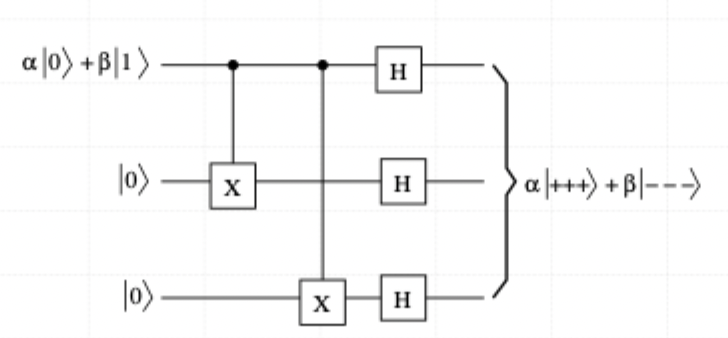
\includegraphics[width=\linewidth]{Quantum Error Correction Phase.png}

\end{multicols*}

\end{document}
